\label{sec:Cloudmigration}
%
\RenewGrass{} has been successfully tested in a local environment.
%
All the required components were hosted on-premise (\Renew{}, Grass GIS and the data).
%
Nevertheless, as soon as the number of tasks increases and the size of data become large, we start facing computing and storage issues.
%
This is due to insufficient resources on the local site.
%
This section presents our vision to deploy the current implementation of the \RenewGrass{} tool onto the Cloud services.
%
First, different possibilities to Cloud-enable an application in general are shortly illustrated.
%
These possibilities are formulated in form of patterns.
%
The illustration is based on the work of \cite{han10} and \cite{leyman09}.
%
They investigate and strive to answer questions like: where to enact the processes? Where to execute the activities? and Where to store the data?
%
Thus the entities taken in account are: (1) the process engine (responsible for the execution and the monitoring of the activities) (2) the activities that need to be executed by the workflow and (3) the Data.
%
Next, we propose an architecture to introduce a new pattern and an appropriate methodology to enable remote execution in the Cloud.
%
This has been also described in a previous work \cite{Bendoukha+15}.
%
\subsection{Migration Patterns}
%
Moving an existing application to the Cloud should be based on a solid strategy.
%
Providing the business management system (or WfMS) or a part in the Cloud raises a series of concerns about ensuring the security of the data and the performance of the system. 
%
For example, Cloud users could lose control on their own data in case of a fully Cloud-based solution. 
%
Some activities, which are not compute-intensive can be executed on-premise rather than moving them to the Cloud. 
%
Unfortunately, this transfer can be time and cost-consuming because of the pay-per-use model and the nature of the workflow tasks.


%
%
%
%
In the following, the patterns from \cite{han10,leyman09} are shortly introduced.
%
%
%
The first pattern designs the traditional scenario where all the components of the workflow system are hosted at the user-side (on-premise).
%
The second scenario represents a case when users already have a workflow engine but the application contains compute or data-intensive activities, so they are moved to the Cloud for acquiring more capabilities and better performance.
%
The third case designs a situation, where the end-users do not have a workflow engine, so they use a Cloud-based workflow engine, which is provided on-demand.
%
In that case, workflow designers can specify transfer requirements of activity execution and data storage, for example, sensitive data and non-compute-intensive activities can be hosted on-premise, and compute-intensive activities and non-sensitive data can be moved to the Cloud \cite{han10}.
%
%
The last scenario presents a situation where all components are hosted in a Cloud and accessed probably from a Web interface.
%
The advantage is that users do not need to install and configure any software on the user side.
%
%
%
%
%
To make an analogy with the elements of our approach, \Renew{} is the process engine, the activities are the geoprocessing tasks (performed by the Grass services), which are related to the satellite images (data).
%
The latter (data and Grass GIS) can be either on-premise or hosted in the Cloud.
%
Based on these elements and the illustration presented above, Fig.~\ref{fig:cloudpatterns} presents an overview of the diverse approaches (patterns) to design our workflow system based on the Cloud technology.
%
\begin{figure}[!t]
    \centering
 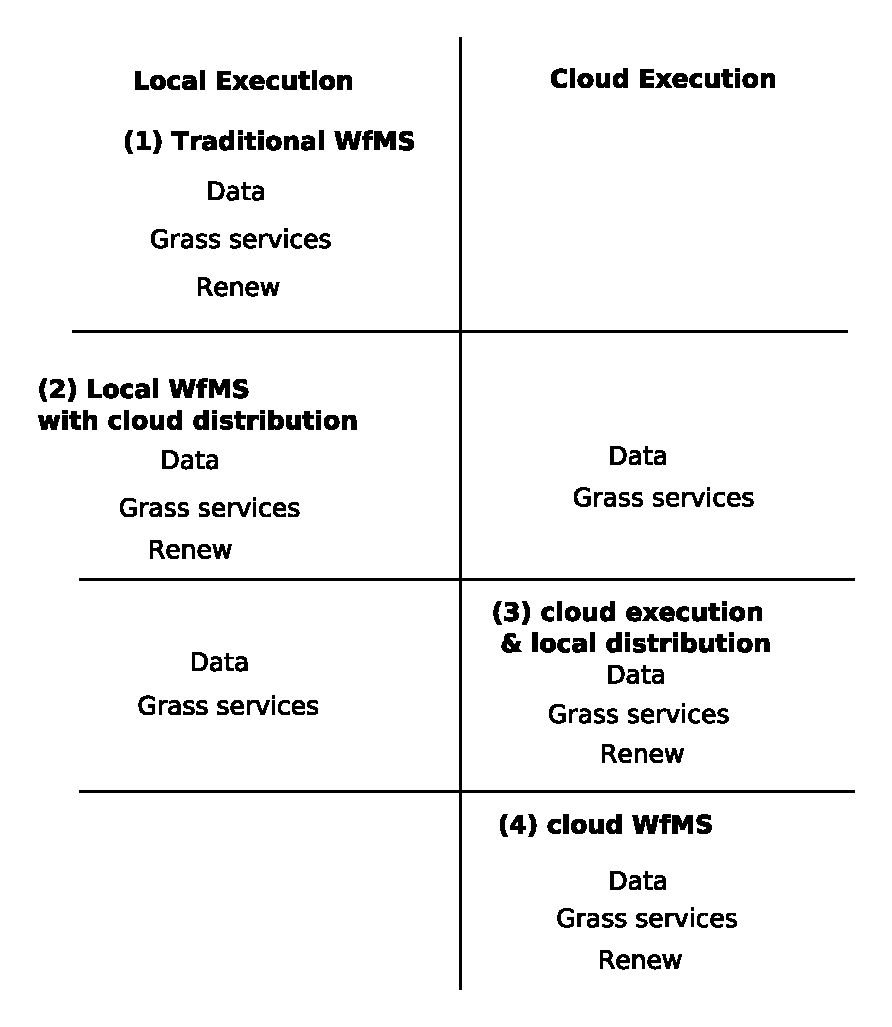
\includegraphics[width=0.68\textwidth,height=0.35\textheight]{images/CloudGrassPatterns}
\caption{Patterns for Cloud-based Workflow Systems (Adapted from \cite{han10})}
\label{fig:cloudpatterns}
\end{figure}



%%%%our work

We have noticed that both \cite{han10} and \cite{leyman09} do not address all possible situations.
%
For instance, the following situation has been not addressed: the process engine is available on the user side but due to circumstances (internal failure, not sufficient compute or storage resources), remote process engines need to be integrated and remotely invoked.
%
Fig. \ref{fig:pattern5} shows approximately how this scenario looks like.
%
Our solution consists on transferring the data and executing the process by another process engine.
%
This is discussed in the following sections. 
%
% 
%
%
\begin{figure}[!t]
    \centering
  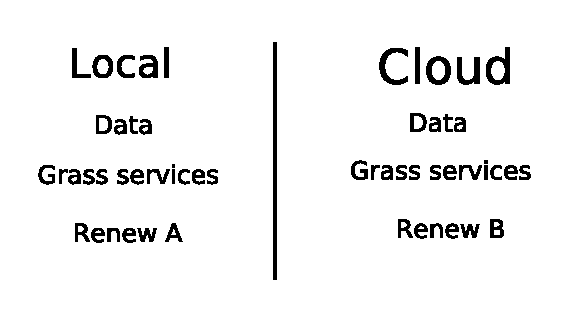
\includegraphics[width=0.48\textwidth,height=0.10\textheight]{images/pattern5}
\caption{A Pattern Designing Multiple Process Engines Integration}
\label{fig:pattern5}
\end{figure}

\subsection{Architecture}
%
Fig. \ref{fig:architecture} shows the architecture to integrate the current implementation into a Cloud system.
%
While \RenewGrass{} is already implemented and successfully integrated in \Renew{} (see section \ref{sec:grassintegration}), most efforts are dedicated now to move the execution of the geoprocessing tasks to the Cloud and the provision of an interface to invoke these services  directly from workflow models.

In our work, we follow an agent-based approach, i.e., many components functionalities are performed by special agents.
%
In summary, the role of each agent used in the approach is described below.
%
\begin{enumerate}
 \item 
 \textit{Workflow Holder Agent}:
 %
 The Workflow holder is the entity that specifies the workflow and in consequence holds the generated Petri net models.
 %
 This entity can be either human or a software component.
 %
 The specification of the image processing workflow is performed using \RenewGrass{}, which provides a modeling palette or downright predefined modeling blocks.
\item 
 \textit{Cloud Portal Agent}:
 %
 provides the \textit{Workflow Holder Agent} a Web portal as a primary interface to the whole system.
 %
 It contains two components: \textit{Cloud Manager} and \textit{Workflow Submission Interface}.
 %
 The latter provides a Web interface to the workflow holders to upload all necessary files to execute the workflow.
 %
 This includes the workflow specification (\Renew{} formats\footnote{\Renew{} supports various file formats saving (XML, .rnw, .sns, etc.)}), input files (images).
 %
 It also serves getting notifications from the \textit{Cloud Broker Agent} about the status of the workflow or the availability of the Cloud provider.
%
The role of the \textit{Cloud Manager} is to control the Cloud instances (start and stop or suspend).

 % 
% 
%
% 
 \item 
 \textit{Cloud Broker Agent}:
 %
 It is a critical component of the architecture, since it is responsible of (i) the evaluation and selection of the Cloud providers that fits the workflow's requirements (e.g., data volume and computing intensities) and (ii) mapping the workflow tasks.% to that Cloud provider to be executed. 
 %
 Both activities require information about the Cloud provider, which are available and provided by the Cloud Repository Agent.
 \item 
 \textit{Cloud Repository Agent}:
 The Cloud repository register the information about the Cloud providers and the state of their services.
 %
 These information are saved in a database and are constantly updated, since they are required by the Cloud Broker Agent.
 %
 To avoid failure scenarios (repository down, loss of data), we use distributed databases, which allows high availability and fault-tolerant persistence.
\item 
 \textit{Cloud Provider Agent}:
The role of this agent is to control the instances and to manage the execution of the tasks.
%
Regularly, the Cloud providers need to update their status and send it to the Cloud Repository Agent.
%
The status concerns both the instance and the services (Grass services).
\end{enumerate}


\begin{figure*}[!t]
    \centering
  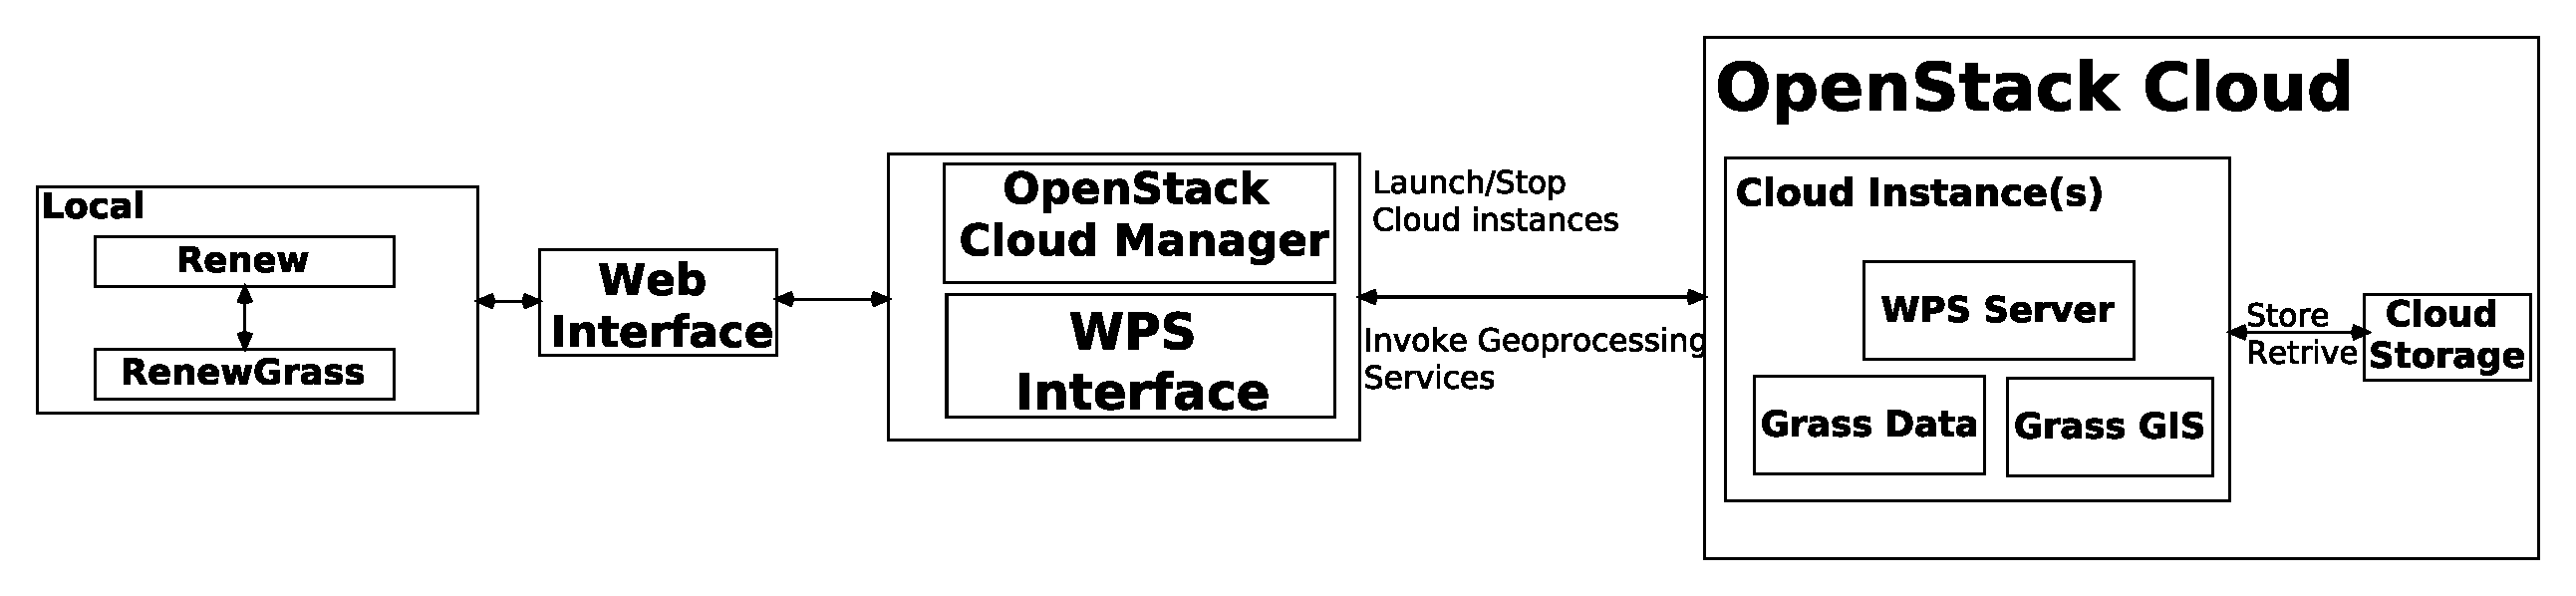
\includegraphics[width=0.98\textwidth,height=0.20\textheight]{images/GrassMigration}
\caption{The Architecture of the Cloud-based Workflow System}
\label{fig:architecture}
\end{figure*}



%%%%%
Concerning the \textit{Cloud Broker Agent}, the evaluation and the selection of the Cloud providers are critical processes for the \textit{Workflow Holders}.
%
In Cloud computing there are various factors impacting the Cloud provider evaluation and selection \cite{Haddad11,Badger+11a} such as: computational capacity, IT security and privacy, reliability and trustworthiness, customization degree and flexibility/scalability, manageability/usability and customer service, geolocations of Cloud infrastructures. 
%
For this, in our work, brokering factors are limited to the computational capacity and the customization degree. 

%
\subsection{Cloud Configuration}
%
Concerning the customization degree, there are some requirements for a successful deployment onto the Cloud.
%
In general, a common procedure to deploy applications onto Cloud services consists of these two main steps: 
%
\begin{enumerate}
 \item 
 \textit{set up the environment}: 
 %
 this mainly consists of the provision of Cloud instances\footnote{The Cloud instances should be in priori customized, i.e, they need to have the Grass GIS as back-end, the WPS server and \Renew{}.
 %
 We assume that the Cloud storage is a service, which is configured by the Cloud provider itself.
 } and the configuration the required softwares properly.
 %
 %
 Essential are the environment variables, which differ from the local implementation such as JAVA configuration for the Web server.
 %
 \item
 \textit{deploy the application}: it consists of the customization of the Cloud instance with the appropriate softwares. 
 %
 For our work, \Renew{} and the Grass GIS should be correctly and properly configured, especially the database and the installation path.
 
 \end{enumerate}
 

%
Furthermore, the Grass commands can be invoked in different ways. 
%
Either through a wrapper like in the original implementation of \RenewGrass{} or provided as Web services.
%
For the latter, we follow a Web-based approach with respect to the Open Geospatial Consortium (OGC) Web Processing Service (WPS) interface specification. 
%
Thus the Grass GIS functionalities are provided as Web services instead of desktop application.
%
To achieve this, we chose the 52North\footnote{http://52north.org/} as a WPS server as well as the wps-grass-bridge\footnote{https://code.google.com/p/wps-grass-bridge/}.

%
\subsection{Execution Scenario}

Considering the proposed architecture and the agent roles described above, a typical deployment scenario is broken into the following steps: 
%
\begin{enumerate}
 \item 
Workflow holders specify their image processing workflows (data and control-flow) using Petri nets for example the NDVI workflow (see section \ref{sec:grassintegration}).
\item 
They send a request to the \textit{Cloud Broker} via the \textit{Cloud Portal}.  
\item
The \textit{Cloud Broker} checks for available Cloud providers, which provide geoprocessing tools (Grass GIS).
%
This information is retrieved from the \textit{Cloud Repository}.
%
\item
The \textit{Cloud Broker} sends a list to the \textit{Workflow Holder} (through the Cloud Portal) to accept or to reject the offer.
\item
If the offer is accepted, the \textit{Workflow Holder} submits the workflow specification (.rnw + .sns) to the selected \textit{Cloud Provider}.
\item
Launch a customized Cloud instance with \Renew{} and Grass GIS running in the background.
\item 
After simulation/execution of the workflow, results (in our prototype it consists of calculating the NDVI value) are transmitted to the \textit{Workflow Holder} through the \textit{Cloud Portal}.
\end{enumerate}

Rejecting an offer does not conclude the execution process immediately. 
%
Since the list transmitted by the \textit{Cloud Broker} is updated constantly,
%
it might be that new Cloud providers are available and fits the requirements.
%
Therefore, from step (3), the process is iterative until the satisfaction of the \textit{Workflow Holder}.
%
Regarding step (5) and (6), \Renew{} supports starting a simulation from the command line.
%
This is possible by using the command \textit{startsimulation (net system) (primary net) [-i]}.
%
The parameters to this command have the following meaning:
%
\begin{itemize}
 \item 
 \textit{net system}: The .sns file.
\item 
 \textit{primary net}: The name of the net, of which a net instance shall be opened when the simulation starts. 
\item
-i: If you set this optional flag, then the simulation is initialized only, that is, the primary
net instance is opened, but the simulation is not started automatically.
\end{itemize}

%In a future paper, we will give a first evaluation of the presented work as well as the progress of the implementation of the components presented in this section.
%
%Furthermore, we have implemented other image processing workflows such as the Normalized Differences Vegetation Index (NDVI). 